\section{Introduction}
\begin{frame}{Update rules}
    
    \begin{itemize}
        \item An update rule is a finite set $X\subseteq\mathbb{Z}^2-\{0\}$
        \item An update family is a finite collection of update rules $\mathscr{U}=\{X\subseteq\mathbb{Z}^2-\{0\}\}$
    \end{itemize}
    
 
\begin{block}{}
   
 $\mathscr{U}$-Bootstrap percolation initialized at $A$ refers to the following process:

 \begin{itemize}
     \item $A_0=A$
     \item $A_{t+1}=A_t\cup \{x\in\mathbb{Z}^2: x+X\subseteq A_t \textit{ for some } X\in\mathscr{U}\}$
 \end{itemize}
 \end{block}
 
 \end{frame}
 \begin{frame}

 \begin{itemize}
 
 
     \item The set $A$ is known as the set of initially infected sites
     \item The closure of $A$ is defined as $[A]=\cup_{t\geq 0} A_t$
     \item The initialization is random i.e. each site (vertex)
     in $\mathbb{Z}^2$ is infected with probability $p$ independently from the other vertices
     \item The process is monotone i.e. if a site gets infected, it stays infected forever
     \item After the initialization, the process is deterministic in the sense that a site will get infected if and only if there is some rule $X$ in $\mathscr{U}$ such that $x+X$ is infected
 \end{itemize}
 


\end{frame}




\begin{frame}{Examples}

\begin{figure}[t]
    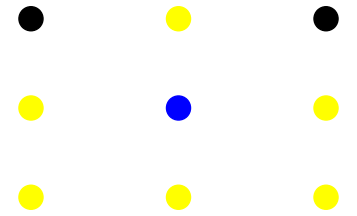
\includegraphics[width=0.18\textwidth]{rgospercrule.png}
    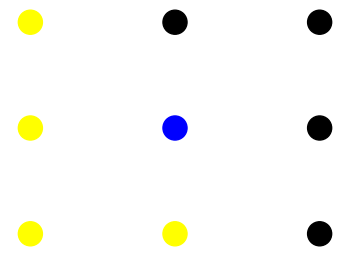
\includegraphics[width=0.15\textwidth]{rgspiralpercrule1.png}
    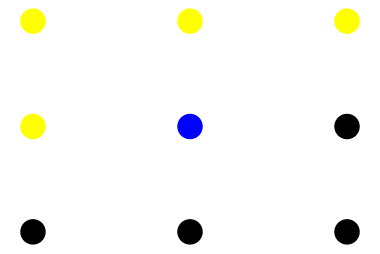
\includegraphics[width=0.17\textwidth]{rgspiralpercrule2.png}
    \caption{Oriented site, rules $U_1$ and $U_2$ for spiral model}
    \label{fig:mesh1}
\end{figure}
\begin{itemize}
    \item r-Neighbour models for r=1,2,3,4
    \item Oriented site $\mathscr{U}=\{(-1,1),(1,1)\}$
    \item Spiral $\mathscr{U}=\{U_1,U_2,U_3,U_4\}$, where 
    $U_1=\{(1,-1),(1,0),(1,1),(0,1)\}$
    \newline
    $U_2=\{(1,-1),(1,0),(-1,-1),(0,-1)\}
    $
    \newline
    $ U_3=-U_1, U_4=-U_2$
    \item Directed triangular bootstrap percolation 
    

\end{itemize}



\end{frame}

\begin{frame}{Stable directions, basic properties}
For a vector $u\in\mathbb{S}^1$, we define $
\mathbb{H}_u=\{x\in\mathbb{Z}^2|<x,u><0\}$.

\begin{block}{Definition}



Given an update family $\mathscr{U}$, a direction $u\in\mathbb{S}^1$ is
\begin{itemize}

    \item stable if $[\mathbb{H}_u]=\mathbb{H}_u$. The set of stable directions is denoted by $\mathscr{S}=\mathscr{S}{U}$
    \item strongly stable if $u\in int\mathscr{S}$
    \item unstable if it is not stable


\end{itemize}
\end{block}


\begin{itemize}
    \item Dichotomy $[\mathbb{H}_u]\in\{\mathbb{H}_u,\mathbb{Z}^2\}$
    \item $\mathscr{S}\subseteq\mathbb{S}^1$ is a set of stable directions for some update familit $\mathscr{U}$ if and only if it can be expressed as a union of closed intervals with rational endpoints\footnote{A direction $u\in\mathbb{S}^1$ is said to be rational if there is a point in the grid $\mathbb{Z}^2\cap\{\lambda u|\lambda\in\mathbb{R}\}$
    1}
    in $\mathbb{S}^1$
\end{itemize}



\end{frame}

\begin{frame}{Classification of $\mathscr{U}$-Bootstrap percolation}
$\mathscr{U}$-bootstrap percolation update families exhibit different properties based on their stable sets. Let $\mathscr{U}$ be an update family with a set of stable directions $\mathscr{S}$
\begin{block}

\begin{itemize}
    \item If there is a open semicircle $C$ such that $\mathscr{S}\cap C=\emptyset$ then $\mathscr{U}$ is said to be \textbf{supercritical}
    \item If every open semicircle $C$ intersects $\mathscr{S}$, but there is an open semicircle $C_0$ that doesn't intersect $int\mathscr{S}$ then $\mathscr{U}$ is said to be \textbf{critical}
    \item If every open semicircle $C$ intersects $int S$ then $\mathscr{U}$ is said to be \textbf{critical}
\end{itemize}

\end{block}

\end{frame}

\begin{frame}{Supercritical and critical families}
\begin{block}{Infection time of the origin}
The infection time of 0 is defined as $\tau_p=\inf\{t\in\mathbb{N}: 0 \in A_t\}$, given that $A_0=A$ is sampled according to a Bernoulli $p$ distribution
\end{block}

\begin{itemize}
    \item For supercritical families, $\tau_p=p^{-\Theta(1)}$ as $p\rightarrow 0$ with high probability
    \item For critical families, $\tau_p=\exp(p^{-\Theta(1)})$ as 
    $p\rightarrow 0$ with high probability
\end{itemize}

Corollary: For supercritical and critical families, $p_c=\inf\{p>0|P_p([A]=\mathbb{Z}^2)=1\}=0$ i.e. for any $p>0$ we have percolation.
\newline
However, for subcritical families the situation is different.

    
\end{frame}